\section{Conclusion}

In theory, with our method we achieve the best of both worlds: having access to the power of SRCGAN’s for the more important parts of the images we superresolution while saving on computation costs by not training on as much noise. However, due to not having the hardware to train an FCN and using third party libraries, our current end product has to re-calculate various values.
Our method is also restricted by the limitations of SRCGAN’s. Since SRCGAN’s
have a fixed nxn sized input, we have to either upscale or downscale our FCN
output in order to pass it to the SRCGAN. Additionally, when we have long or
tall subjects, like a giraffe, we need to pass additional background information
that we know isn’t our subject into the SRCGAN (as seen in Figure \ref{fig:giraffe}), resulting in
noise when both training and running the SRCGAN.

\begin{figure}
    \centering
    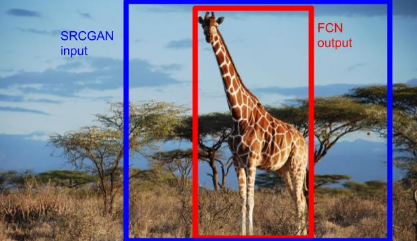
\includegraphics[width=0.45\textwidth]{images/giraffe.png}
    \caption{An example of an inefficiency with our method. Although the FCN knows the giraffe is bounded within the red box, due to the nature of SRCGAN's we are forced to pass the blue box, essentially wasting computation.}
    \label{fig:giraffe}
\end{figure}


Another issue with our method is when multiple subjects overlap. Since we run our SRCGAN for each image we classify, any overlap is enhanced multiple times, causing unnecessary calculation as seen in Figure \ref{fig:crossover}. As such, our method would not work well when the FCN classifiers more area as subjects than the size of the original image.

\begin{figure}
    \centering
    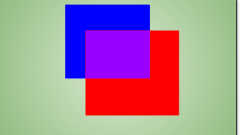
\includegraphics[width=0.45\textwidth]{images/crossover.png}
    \caption{If the FCN classifies the red area as one class and the blue are as another, the purple area is run through the SRCGAN twice.}
    \label{fig:crossover}
\end{figure}


\section{Future Work}

Our goal for Context Aware Super Resolution is to one day use it for video compression. The end goal would be to have . While current research has shown potential for video compression using super resolution, nothing pratical has yet to be created [1][2]. We hope to create a refined version of our method that could potentially be used for compression videos with a low subject count (Figure \ref{fig:compression})


\begin{figure}
    \centering
    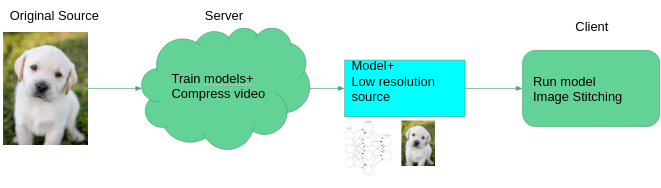
\includegraphics[width=1\textwidth]{images/compression.png}
    \caption{A potential server-client model for video compression using Context Aware Super Resolution}
    \label{fig:compression}
\end{figure}

